\begin{multicols*}{2}
\section{\codeinlineSect{tcolorbox} 代码块测试}

\subsection{\codeinlineSectSub{tcolorbox} 代码块测试}

\subsubsection{\codeinlineSectSubSub{tcolorbox} 代码块测试}

\begin{codefence}[./fgmain.tex]\Highlight{4-5,10}\Mode{listing and text}\ %This space is mandatory, otherwise the first command will be gobbled.
% 代码块中高亮行的行号也能被高亮 。
% 代码来自 https://tex.stackexchange.com/questions/741923
% 相关的库 : minted , fbextra , fancyvrb , etoolbox
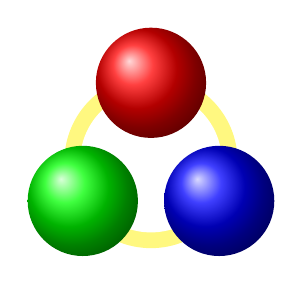
\begin{tikzpicture}
\path[fill=yellow!50!white] (0,0) circle (11mm);
\path[fill=white] (0,0) circle (9mm);
\foreach \w/\c in {90/red,210/green,330/blue}
{\path[shading=ball,ball color=\c] (\w:1cm) circle (7mm);}
\end{tikzpicture}
% import Lib
% import Control.Lens
\end{codefence}

\begin{codefence}[test.hs]\Syntax{haskell}\Highlight{1-4,10}
module Main where

import Lib
import 脎\codeHL{Control}吡Control.Lens 

main :: IO ()
main = someFunc 

lst = [x| x <- ['a'..'z']] 
-- 注意左侧行号
\end{codefence}

左侧 \LaTeX 语言高亮似乎有些问题,这个应该是 Pygments 的锅。

% \vfill\null\columnbreak

\begin{codefence}\Syntax{racket}
;; 过程合约 :  in-S? : Natural   → Bool
;; 过程用途 : (in-S?     n   )   = #t 仅当 n 属于 S , 否则为 #f
;; 实参语法 :          Natural ::=  0 | (succ Natural)
(define in-S? 
  (lambda (n)
    (if (zero? n) #t
        (if (>= (- n 3) 0) (in-S? (- n 3))
            #f))))
\end{codefence}

泥濠!我是沉积岩!下面是一段一段测试文字:%
\codeinline[haskell]{lst = [x| x <- }
\codeinline[haskell]{['a'..'g']] -- by 沉积岩}
\codeinline{tcolorbox}
\end{multicols*}